% Options for packages loaded elsewhere
% Options for packages loaded elsewhere
\PassOptionsToPackage{unicode}{hyperref}
\PassOptionsToPackage{hyphens}{url}
\PassOptionsToPackage{dvipsnames,svgnames,x11names}{xcolor}
%
\documentclass[
  a4paper,
]{report}
\usepackage{xcolor}
\usepackage[left=24mm,right=24mm,top=22mm,bottom=24mm]{geometry}
\usepackage{amsmath,amssymb}
\setcounter{secnumdepth}{5}
\usepackage{iftex}
\ifPDFTeX
  \usepackage[T1]{fontenc}
  \usepackage[utf8]{inputenc}
  \usepackage{textcomp} % provide euro and other symbols
\else % if luatex or xetex
  \usepackage{unicode-math} % this also loads fontspec
  \defaultfontfeatures{Scale=MatchLowercase}
  \defaultfontfeatures[\rmfamily]{Ligatures=TeX,Scale=1}
\fi
\usepackage{lmodern}
\ifPDFTeX\else
  % xetex/luatex font selection
\fi
% Use upquote if available, for straight quotes in verbatim environments
\IfFileExists{upquote.sty}{\usepackage{upquote}}{}
\IfFileExists{microtype.sty}{% use microtype if available
  \usepackage[]{microtype}
  \UseMicrotypeSet[protrusion]{basicmath} % disable protrusion for tt fonts
}{}
\makeatletter
\@ifundefined{KOMAClassName}{% if non-KOMA class
  \IfFileExists{parskip.sty}{%
    \usepackage{parskip}
  }{% else
    \setlength{\parindent}{0pt}
    \setlength{\parskip}{6pt plus 2pt minus 1pt}}
}{% if KOMA class
  \KOMAoptions{parskip=half}}
\makeatother
% Make \paragraph and \subparagraph free-standing
\makeatletter
\ifx\paragraph\undefined\else
  \let\oldparagraph\paragraph
  \renewcommand{\paragraph}{
    \@ifstar
      \xxxParagraphStar
      \xxxParagraphNoStar
  }
  \newcommand{\xxxParagraphStar}[1]{\oldparagraph*{#1}\mbox{}}
  \newcommand{\xxxParagraphNoStar}[1]{\oldparagraph{#1}\mbox{}}
\fi
\ifx\subparagraph\undefined\else
  \let\oldsubparagraph\subparagraph
  \renewcommand{\subparagraph}{
    \@ifstar
      \xxxSubParagraphStar
      \xxxSubParagraphNoStar
  }
  \newcommand{\xxxSubParagraphStar}[1]{\oldsubparagraph*{#1}\mbox{}}
  \newcommand{\xxxSubParagraphNoStar}[1]{\oldsubparagraph{#1}\mbox{}}
\fi
\makeatother

\usepackage{color}
\usepackage{fancyvrb}
\newcommand{\VerbBar}{|}
\newcommand{\VERB}{\Verb[commandchars=\\\{\}]}
\DefineVerbatimEnvironment{Highlighting}{Verbatim}{commandchars=\\\{\}}
% Add ',fontsize=\small' for more characters per line
\usepackage{framed}
\definecolor{shadecolor}{RGB}{241,243,245}
\newenvironment{Shaded}{\begin{snugshade}}{\end{snugshade}}
\newcommand{\AlertTok}[1]{\textcolor[rgb]{0.68,0.00,0.00}{#1}}
\newcommand{\AnnotationTok}[1]{\textcolor[rgb]{0.37,0.37,0.37}{#1}}
\newcommand{\AttributeTok}[1]{\textcolor[rgb]{0.40,0.45,0.13}{#1}}
\newcommand{\BaseNTok}[1]{\textcolor[rgb]{0.68,0.00,0.00}{#1}}
\newcommand{\BuiltInTok}[1]{\textcolor[rgb]{0.00,0.23,0.31}{#1}}
\newcommand{\CharTok}[1]{\textcolor[rgb]{0.13,0.47,0.30}{#1}}
\newcommand{\CommentTok}[1]{\textcolor[rgb]{0.37,0.37,0.37}{#1}}
\newcommand{\CommentVarTok}[1]{\textcolor[rgb]{0.37,0.37,0.37}{\textit{#1}}}
\newcommand{\ConstantTok}[1]{\textcolor[rgb]{0.56,0.35,0.01}{#1}}
\newcommand{\ControlFlowTok}[1]{\textcolor[rgb]{0.00,0.23,0.31}{\textbf{#1}}}
\newcommand{\DataTypeTok}[1]{\textcolor[rgb]{0.68,0.00,0.00}{#1}}
\newcommand{\DecValTok}[1]{\textcolor[rgb]{0.68,0.00,0.00}{#1}}
\newcommand{\DocumentationTok}[1]{\textcolor[rgb]{0.37,0.37,0.37}{\textit{#1}}}
\newcommand{\ErrorTok}[1]{\textcolor[rgb]{0.68,0.00,0.00}{#1}}
\newcommand{\ExtensionTok}[1]{\textcolor[rgb]{0.00,0.23,0.31}{#1}}
\newcommand{\FloatTok}[1]{\textcolor[rgb]{0.68,0.00,0.00}{#1}}
\newcommand{\FunctionTok}[1]{\textcolor[rgb]{0.28,0.35,0.67}{#1}}
\newcommand{\ImportTok}[1]{\textcolor[rgb]{0.00,0.46,0.62}{#1}}
\newcommand{\InformationTok}[1]{\textcolor[rgb]{0.37,0.37,0.37}{#1}}
\newcommand{\KeywordTok}[1]{\textcolor[rgb]{0.00,0.23,0.31}{\textbf{#1}}}
\newcommand{\NormalTok}[1]{\textcolor[rgb]{0.00,0.23,0.31}{#1}}
\newcommand{\OperatorTok}[1]{\textcolor[rgb]{0.37,0.37,0.37}{#1}}
\newcommand{\OtherTok}[1]{\textcolor[rgb]{0.00,0.23,0.31}{#1}}
\newcommand{\PreprocessorTok}[1]{\textcolor[rgb]{0.68,0.00,0.00}{#1}}
\newcommand{\RegionMarkerTok}[1]{\textcolor[rgb]{0.00,0.23,0.31}{#1}}
\newcommand{\SpecialCharTok}[1]{\textcolor[rgb]{0.37,0.37,0.37}{#1}}
\newcommand{\SpecialStringTok}[1]{\textcolor[rgb]{0.13,0.47,0.30}{#1}}
\newcommand{\StringTok}[1]{\textcolor[rgb]{0.13,0.47,0.30}{#1}}
\newcommand{\VariableTok}[1]{\textcolor[rgb]{0.07,0.07,0.07}{#1}}
\newcommand{\VerbatimStringTok}[1]{\textcolor[rgb]{0.13,0.47,0.30}{#1}}
\newcommand{\WarningTok}[1]{\textcolor[rgb]{0.37,0.37,0.37}{\textit{#1}}}

\usepackage{longtable,booktabs,array}
\usepackage{calc} % for calculating minipage widths
% Correct order of tables after \paragraph or \subparagraph
\usepackage{etoolbox}
\makeatletter
\patchcmd\longtable{\par}{\if@noskipsec\mbox{}\fi\par}{}{}
\makeatother
% Allow footnotes in longtable head/foot
\IfFileExists{footnotehyper.sty}{\usepackage{footnotehyper}}{\usepackage{footnote}}
\makesavenoteenv{longtable}
\usepackage{graphicx}
\makeatletter
\newsavebox\pandoc@box
\newcommand*\pandocbounded[1]{% scales image to fit in text height/width
  \sbox\pandoc@box{#1}%
  \Gscale@div\@tempa{\textheight}{\dimexpr\ht\pandoc@box+\dp\pandoc@box\relax}%
  \Gscale@div\@tempb{\linewidth}{\wd\pandoc@box}%
  \ifdim\@tempb\p@<\@tempa\p@\let\@tempa\@tempb\fi% select the smaller of both
  \ifdim\@tempa\p@<\p@\scalebox{\@tempa}{\usebox\pandoc@box}%
  \else\usebox{\pandoc@box}%
  \fi%
}
% Set default figure placement to htbp
\def\fps@figure{htbp}
\makeatother





\setlength{\emergencystretch}{3em} % prevent overfull lines

\providecommand{\tightlist}{%
  \setlength{\itemsep}{0pt}\setlength{\parskip}{0pt}}



 


% Better typography and table control
\usepackage{booktabs}
\usepackage{array}
\usepackage{longtable}
\usepackage{tabularx}
\usepackage{adjustbox}
\usepackage{pdflscape}
\usepackage{microtype}
% Global table breathing room
\setlength{\extrarowheight}{2pt}
\renewcommand{\arraystretch}{1.15}
\makeatletter
\@ifpackageloaded{tcolorbox}{}{\usepackage[skins,breakable]{tcolorbox}}
\@ifpackageloaded{fontawesome5}{}{\usepackage{fontawesome5}}
\definecolor{quarto-callout-color}{HTML}{909090}
\definecolor{quarto-callout-note-color}{HTML}{0758E5}
\definecolor{quarto-callout-important-color}{HTML}{CC1914}
\definecolor{quarto-callout-warning-color}{HTML}{EB9113}
\definecolor{quarto-callout-tip-color}{HTML}{00A047}
\definecolor{quarto-callout-caution-color}{HTML}{FC5300}
\definecolor{quarto-callout-color-frame}{HTML}{acacac}
\definecolor{quarto-callout-note-color-frame}{HTML}{4582ec}
\definecolor{quarto-callout-important-color-frame}{HTML}{d9534f}
\definecolor{quarto-callout-warning-color-frame}{HTML}{f0ad4e}
\definecolor{quarto-callout-tip-color-frame}{HTML}{02b875}
\definecolor{quarto-callout-caution-color-frame}{HTML}{fd7e14}
\makeatother
\makeatletter
\@ifpackageloaded{bookmark}{}{\usepackage{bookmark}}
\makeatother
\makeatletter
\@ifpackageloaded{caption}{}{\usepackage{caption}}
\AtBeginDocument{%
\ifdefined\contentsname
  \renewcommand*\contentsname{Table of contents}
\else
  \newcommand\contentsname{Table of contents}
\fi
\ifdefined\listfigurename
  \renewcommand*\listfigurename{List of Figures}
\else
  \newcommand\listfigurename{List of Figures}
\fi
\ifdefined\listtablename
  \renewcommand*\listtablename{List of Tables}
\else
  \newcommand\listtablename{List of Tables}
\fi
\ifdefined\figurename
  \renewcommand*\figurename{Figure}
\else
  \newcommand\figurename{Figure}
\fi
\ifdefined\tablename
  \renewcommand*\tablename{Table}
\else
  \newcommand\tablename{Table}
\fi
}
\@ifpackageloaded{float}{}{\usepackage{float}}
\floatstyle{ruled}
\@ifundefined{c@chapter}{\newfloat{codelisting}{h}{lop}}{\newfloat{codelisting}{h}{lop}[chapter]}
\floatname{codelisting}{Listing}
\newcommand*\listoflistings{\listof{codelisting}{List of Listings}}
\makeatother
\makeatletter
\usepackage{pdflscape}
\makeatother
\makeatletter
\makeatother
\makeatletter
\@ifpackageloaded{caption}{}{\usepackage{caption}}
\@ifpackageloaded{subcaption}{}{\usepackage{subcaption}}
\makeatother
\usepackage{bookmark}
\IfFileExists{xurl.sty}{\usepackage{xurl}}{} % add URL line breaks if available
\urlstyle{same}
\hypersetup{
  pdftitle={After Cognition: Visual Companion},
  pdfauthor={Magnús Már Smárason},
  colorlinks=true,
  linkcolor={blue},
  filecolor={Maroon},
  citecolor={Blue},
  urlcolor={Blue},
  pdfcreator={LaTeX via pandoc}}


\title{After Cognition: Visual Companion}
\usepackage{etoolbox}
\makeatletter
\providecommand{\subtitle}[1]{% add subtitle to \maketitle
  \apptocmd{\@title}{\par {\large #1 \par}}{}{}
}
\makeatother
\subtitle{All Figures, Tables, and Visual Elements}
\author{Magnús Már Smárason}
\date{2025-08-10}
\begin{document}
\maketitle

\renewcommand*\contentsname{Table of contents}
{
\hypersetup{linkcolor=}
\setcounter{tocdepth}{2}
\tableofcontents
}

\bookmarksetup{startatroot}

\chapter*{Preface}\label{preface}
\addcontentsline{toc}{chapter}{Preface}

\markboth{Preface}{Preface}

This companion volume collects all visual elements from ``After
Cognition: Human Value in the Age of Irreducibility'' for easy reference
and improved rendering quality.

The visuals are organized by the parts of the main manuscript:

\begin{itemize}
\tightlist
\item
  \textbf{Part I}: Economic tables and displacement data
\item
  \textbf{Part II}: The Three Domains framework and summary tables\\
\item
  \textbf{Part III}: Market cases, LVDC examples, and cultivation
  practices
\item
  \textbf{Part IV}: Implementation frameworks and case examples
\item
  \textbf{Appendix}: Additional visual materials
\end{itemize}

Each visual element is presented with its original context and caption
for reference.

\section*{How to Use This Companion}\label{how-to-use-this-companion}
\addcontentsline{toc}{section}{How to Use This Companion}

\markright{How to Use This Companion}

\begin{enumerate}
\def\labelenumi{\arabic{enumi}.}
\tightlist
\item
  \textbf{For Quick Reference}: Use the table of contents to jump
  directly to specific visuals
\item
  \textbf{For Presentations}: All images are available in high-quality
  formats in the \texttt{images/} folder
\item
  \textbf{For Further Analysis}: Tables are presented in clean, copyable
  formats
\end{enumerate}

All visual elements maintain their original numbering and references
from the main manuscript.

\bookmarksetup{startatroot}

\chapter{Part I: Economic and Existential Imperative
Visuals}\label{part-i-economic-and-existential-imperative-visuals}

This chapter contains all tables and visual elements from Part I of the
main manuscript.

\section{Economic Model Comparison}\label{economic-model-comparison}

\subsection{Table 1.1 --- Traditional SaaS vs AI/COGSware
Economics}\label{table-1.1-traditional-saas-vs-aicogsware-economics}

\begin{longtable}[]{@{}
  >{\raggedright\arraybackslash}p{(\linewidth - 4\tabcolsep) * \real{0.2763}}
  >{\raggedright\arraybackslash}p{(\linewidth - 4\tabcolsep) * \real{0.3947}}
  >{\raggedright\arraybackslash}p{(\linewidth - 4\tabcolsep) * \real{0.3289}}@{}}
\toprule\noalign{}
\begin{minipage}[b]{\linewidth}\raggedright
\textbf{Dimension}
\end{minipage} & \begin{minipage}[b]{\linewidth}\raggedright
\textbf{Traditional SaaS}
\end{minipage} & \begin{minipage}[b]{\linewidth}\raggedright
\textbf{AI/COGSware}
\end{minipage} \\
\midrule\noalign{}
\endhead
\bottomrule\noalign{}
\endlastfoot
Cost Structure & Fixed infrastructure & Variable compute \\
Gross Margins & 80--90\% & 50--70\% \\
Pricing Model & Per seat/month & Per token/query \\
Scaling & \textbf{Near-zero marginal cost} & \textbf{Linear compute
costs} \\
\end{longtable}

\emph{Economic comparison of Traditional SaaS vs AI/COGSware
ecosystems.}

\begin{tcolorbox}[enhanced jigsaw, toprule=.15mm, rightrule=.15mm, breakable, opacitybacktitle=0.6, colframe=quarto-callout-important-color-frame, colback=white, titlerule=0mm, arc=.35mm, leftrule=.75mm, opacityback=0, colbacktitle=quarto-callout-important-color!10!white, bottomrule=.15mm, coltitle=black, toptitle=1mm, bottomtitle=1mm, title=\textcolor{quarto-callout-important-color}{\faExclamation}\hspace{0.5em}{Important}, left=2mm]

This table illustrates the shift from fixed-cost software to
variable-cost AI computation with direct effects on margins and value
capture.

\end{tcolorbox}

\section{Stratified Reality of
Displacement}\label{stratified-reality-of-displacement}

\subsection{Table 1.2 --- Stratified Displacement Snapshot
(Illustrative)}\label{table-1.2-stratified-displacement-snapshot-illustrative}

\begin{longtable}[]{@{}
  >{\raggedright\arraybackslash}p{(\linewidth - 6\tabcolsep) * \real{0.1901}}
  >{\raggedright\arraybackslash}p{(\linewidth - 6\tabcolsep) * \real{0.3223}}
  >{\raggedright\arraybackslash}p{(\linewidth - 6\tabcolsep) * \real{0.2066}}
  >{\raggedright\arraybackslash}p{(\linewidth - 6\tabcolsep) * \real{0.2810}}@{}}
\toprule\noalign{}
\begin{minipage}[b]{\linewidth}\raggedright
\textbf{Group / Domain}
\end{minipage} & \begin{minipage}[b]{\linewidth}\raggedright
\textbf{Indicator}
\end{minipage} & \begin{minipage}[b]{\linewidth}\raggedright
\textbf{Approx. Magnitude}
\end{minipage} & \begin{minipage}[b]{\linewidth}\raggedright
\textbf{Source}
\end{minipage} \\
\midrule\noalign{}
\endhead
\bottomrule\noalign{}
\endlastfoot
Hispanic workers & High-risk occupations overrepresentation & 22 of top
30 & {[}@baboolall2018automation{]} \\
Hispanic workers (6 states) & High automation-risk workers & 7.1 M (≈
40\% workforce) & {[}@dominguez2020latinos{]} \\
Black workers & Displacement rate (potential) & ≈ 23.1\% &
{[}@cook2019future{]} \\
White workers & Displacement rate (potential) & ≈ 22.4\% &
{[}@cook2019future{]} \\
Surveillance bias & Wrongful arrests via facial recognition &
Predominantly Black men (cases) & {[}@aclu2024surveillance{]} \\
Reskilling barrier & Lower retraining participation & Qualitative
disadvantage & {[}@nsc2023digital; @urban2023jobquality{]} \\
\end{longtable}

\emph{Illustrative, heterogeneous sources; magnitudes are not directly
comparable across methodologies.}

\begin{tcolorbox}[enhanced jigsaw, toprule=.15mm, rightrule=.15mm, breakable, opacitybacktitle=0.6, colframe=quarto-callout-warning-color-frame, colback=white, titlerule=0mm, arc=.35mm, leftrule=.75mm, opacityback=0, colbacktitle=quarto-callout-warning-color!10!white, bottomrule=.15mm, coltitle=black, toptitle=1mm, bottomtitle=1mm, title=\textcolor{quarto-callout-warning-color}{\faExclamationTriangle}\hspace{0.5em}{Warning}, left=2mm]

This data reveals how the commoditization crisis falls
disproportionately on already marginalized communities. Any proposed
solutions must address these disparities directly.

\end{tcolorbox}

\section{Key Insights from Part I
Visuals}\label{key-insights-from-part-i-visuals}

\begin{enumerate}
\def\labelenumi{\arabic{enumi}.}
\tightlist
\item
  \textbf{Economic Inversion}: The shift from fixed to variable costs
  fundamentally changes the economics of cognitive work
\item
  \textbf{Unequal Impact}: Automation displacement follows existing
  patterns of inequality
\item
  \textbf{Systemic Nature}: The crisis is not merely technological but
  deeply social and economic
\end{enumerate}

These visuals establish the empirical foundation for the Value
Concentration Hypothesis developed in subsequent parts.

\bookmarksetup{startatroot}

\chapter{Part II: Lifeworld Cartography
Visuals}\label{part-ii-lifeworld-cartography-visuals}

This chapter contains the core visual framework of the thesis - the
Three Domains of Irreducible Human Value.

\section{The Three Domains Framework}\label{the-three-domains-framework}

\subsection{Figure 2.1 --- The Three Domains of Irreducible Human
Value}\label{figure-2.1-the-three-domains-of-irreducible-human-value}

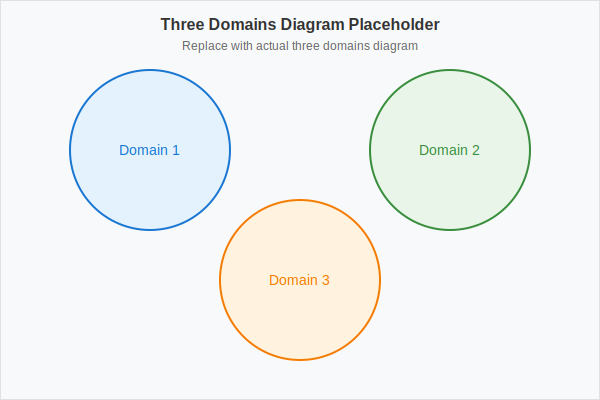
\includegraphics[width=1\linewidth,height=\textheight,keepaspectratio]{index_files/mediabag/images/three-domains-diagram.pdf}

\emph{At the intersection of Presence (embodied self), Cohesion
(intersubjective we), and Meaning (narrative arc) lies the irreducible
core of human experience that remains beyond computational replication.}

\begin{tcolorbox}[enhanced jigsaw, toprule=.15mm, rightrule=.15mm, breakable, opacitybacktitle=0.6, colframe=quarto-callout-tip-color-frame, colback=white, titlerule=0mm, arc=.35mm, leftrule=.75mm, opacityback=0, colbacktitle=quarto-callout-tip-color!10!white, bottomrule=.15mm, coltitle=black, toptitle=1mm, bottomtitle=1mm, title=\textcolor{quarto-callout-tip-color}{\faLightbulb}\hspace{0.5em}{Tip}, left=2mm]

This Venn diagram represents the thesis's central theoretical
contribution. The overlapping areas indicate how these domains
interpenetrate and reinforce each other in lived experience.

\end{tcolorbox}

\section{Domains Summary Table}\label{domains-summary-table}

\subsection{Table 2.1 --- Three Domains: Definitions, Indicators,
Examples}\label{table-2.1-three-domains-definitions-indicators-examples}

\begin{longtable}[]{@{}
  >{\raggedright\arraybackslash}p{(\linewidth - 4\tabcolsep) * \real{0.3333}}
  >{\raggedright\arraybackslash}p{(\linewidth - 4\tabcolsep) * \real{0.3333}}
  >{\raggedright\arraybackslash}p{(\linewidth - 4\tabcolsep) * \real{0.3333}}@{}}
\toprule\noalign{}
\begin{minipage}[b]{\linewidth}\raggedright
\textbf{Domain}
\end{minipage} & \begin{minipage}[b]{\linewidth}\raggedright
\textbf{Operational Indicators (examples)}
\end{minipage} & \begin{minipage}[b]{\linewidth}\raggedright
\textbf{Everyday Examples}
\end{minipage} \\
\midrule\noalign{}
\endhead
\bottomrule\noalign{}
\endlastfoot
Presence & Interoception (MAIA); sustained attention (MAAS/FFMQ);
proprioceptive accuracy & Nurse sensing fever break; mechanic diagnosing
by vibration; mindful walking \\
Cohesion & Trust scale change; rupture--repair latency; reciprocity
index & Sweat-lodge/choral resonance; ``smoke break'' ritual; conflict
repair \\
Meaning & McAdams coherence; PTGI; purpose alignment & Reframing
migration story; post-injury union safety leadership \\
\end{longtable}

\emph{Indicators are illustrative and would require full psychometric
development before use.}

\begin{tcolorbox}[enhanced jigsaw, toprule=.15mm, rightrule=.15mm, breakable, opacitybacktitle=0.6, colframe=quarto-callout-note-color-frame, colback=white, titlerule=0mm, arc=.35mm, leftrule=.75mm, opacityback=0, colbacktitle=quarto-callout-note-color!10!white, bottomrule=.15mm, coltitle=black, toptitle=1mm, bottomtitle=1mm, title=\textcolor{quarto-callout-note-color}{\faInfo}\hspace{0.5em}{Measurement Note}, left=2mm]

The operational indicators listed represent potential empirical
approaches to validating these domains. Full psychometric development
would be required before practical application.

\end{tcolorbox}

\section{Cultural Variations in Domain
Expression}\label{cultural-variations-in-domain-expression}

While the three domains appear universal, their specific expressions
vary across cultures:

\begin{itemize}
\tightlist
\item
  \textbf{Western emphasis}: Individual presence, dyadic trust, personal
  narrative
\item
  \textbf{Ubuntu philosophy}: Collective presence, communal bonds,
  shared story
\item
  \textbf{Buddhist traditions}: Non-self awareness, compassionate
  connection, liberation narrative
\item
  \textbf{Indigenous worldviews}: Land-based presence, kinship networks,
  cyclical meaning
\end{itemize}

\section{Key Insights from Part II
Visuals}\label{key-insights-from-part-ii-visuals}

\begin{enumerate}
\def\labelenumi{\arabic{enumi}.}
\tightlist
\item
  \textbf{Interdependence}: The domains are not isolated capacities but
  mutually reinforcing aspects of human experience
\item
  \textbf{Measurability}: While irreducible to computation, these
  domains can be empirically validated
\item
  \textbf{Universality with Variation}: The framework captures human
  universals while allowing cultural specificity
\end{enumerate}

This visual framework provides the theoretical foundation for
understanding where human value concentrates as AI commoditizes
cognitive tasks.

\bookmarksetup{startatroot}

\chapter{Part III: Value Concentration Gradient
Visuals}\label{part-iii-value-concentration-gradient-visuals}

This chapter contains market cases, economic models, and the Life-Value
Development Compass (LVDC) framework from Part III.

\section{Market Evidence for Value
Concentration}\label{market-evidence-for-value-concentration}

\subsection{Market Case 1: Live Performance
vs.~Streaming}\label{market-case-1-live-performance-vs.-streaming}

\section{The Premium Structure}

\begin{longtable}[]{@{}
  >{\raggedright\arraybackslash}p{(\linewidth - 6\tabcolsep) * \real{0.1930}}
  >{\raggedright\arraybackslash}p{(\linewidth - 6\tabcolsep) * \real{0.1930}}
  >{\raggedright\arraybackslash}p{(\linewidth - 6\tabcolsep) * \real{0.3158}}
  >{\raggedright\arraybackslash}p{(\linewidth - 6\tabcolsep) * \real{0.2982}}@{}}
\toprule\noalign{}
\begin{minipage}[b]{\linewidth}\raggedright
Dimension
\end{minipage} & \begin{minipage}[b]{\linewidth}\raggedright
Streaming
\end{minipage} & \begin{minipage}[b]{\linewidth}\raggedright
Live Performance
\end{minipage} & \begin{minipage}[b]{\linewidth}\raggedright
Premium Multiple
\end{minipage} \\
\midrule\noalign{}
\endhead
\bottomrule\noalign{}
\endlastfoot
\textbf{Cost to Consumer} & \$10/month unlimited & \$250/ticket average
& 25x per event \\
\textbf{Artist Revenue} & \$0.003-0.008 per stream & \$100-150 per
ticket & 12,500-50,000x \\
\textbf{Experience Duration} & 3-4 minutes & 2-3 hours & Similar \\
\textbf{Repeatability} & Infinite & Once & ∞ \\
\textbf{Global Reach} & Billions & Thousands & 0.000001x \\
\end{longtable}

\section{Key Insights}

The music industry illustrates authenticity premiums in action. While
streaming services offer perfect audio quality and infinite
accessibility at near-zero marginal cost, live concert revenues have
grown substantially, with the global concert industry reaching
\textbf{\$31.5 billion in 2023} despite streaming's dominance.

Taylor Swift's Eras Tour exemplifies this premium, grossing over
\textbf{\$1 billion} with average ticket prices exceeding \$250, while
streaming royalties average fractions of a cent per play.

The premium---orders of magnitude higher---pays not for superior audio
but for \textbf{unrepeatable presence}: the artist's mortality performed
in real-time, the collective effervescence of shared experience, the
possibility that this performance might deviate from script.

\subsection{Market Case 2: Boutique Therapy vs.~AI
Chatbots}\label{market-case-2-boutique-therapy-vs.-ai-chatbots}

\section{Cost Comparison}

\begin{longtable}[]{@{}
  >{\raggedright\arraybackslash}p{(\linewidth - 8\tabcolsep) * \real{0.2000}}
  >{\raggedright\arraybackslash}p{(\linewidth - 8\tabcolsep) * \real{0.2000}}
  >{\raggedright\arraybackslash}p{(\linewidth - 8\tabcolsep) * \real{0.2000}}
  >{\raggedright\arraybackslash}p{(\linewidth - 8\tabcolsep) * \real{0.2143}}
  >{\raggedright\arraybackslash}p{(\linewidth - 8\tabcolsep) * \real{0.1857}}@{}}
\toprule\noalign{}
\begin{minipage}[b]{\linewidth}\raggedright
Service Type
\end{minipage} & \begin{minipage}[b]{\linewidth}\raggedright
Monthly Cost
\end{minipage} & \begin{minipage}[b]{\linewidth}\raggedright
Availability
\end{minipage} & \begin{minipage}[b]{\linewidth}\raggedright
Response Time
\end{minipage} & \begin{minipage}[b]{\linewidth}\raggedright
Consistency
\end{minipage} \\
\midrule\noalign{}
\endhead
\bottomrule\noalign{}
\endlastfoot
\textbf{AI Chatbots} (Woebot, Replika) & \$10-20 & 24/7 & Immediate &
100\% protocol adherence \\
\textbf{Human Therapists} & \$600-1200 (4 sessions) & Limited hours &
1-2 week wait & Variable, adaptive \\
\textbf{Premium Ratio} & 30-60x & 0.1x & 0.001x & Variable \\
\end{longtable}

\section{Value Proposition Analysis}

Mental health services demonstrate similar dynamics. While AI therapy
chatbots offer round-the-clock availability at minimal cost, human
therapists charging \textbf{\$150-300/hour} report waitlists despite AI
alternatives.

The premium doesn't purchase superior CBT protocols---AI often adheres
more consistently to evidence-based practices. Instead, it buys
\textbf{relationship with a consciousness} that has genuinely suffered,
recovered, and chosen to transmute that experience into healing
presence.

This therapeutic alliance, grounded in mutual vulnerability, remains
architecturally impossible for systems without stakes in existence.

\section{The Life-Value Development Compass
(LVDC)}\label{the-life-value-development-compass-lvdc}

\subsection{Table 3.1: Illustrative LVDC Sample Items - Theoretical
Examples}\label{table-3.1-illustrative-lvdc-sample-items---theoretical-examples}

\begin{tcolorbox}[enhanced jigsaw, toprule=.15mm, rightrule=.15mm, breakable, opacitybacktitle=0.6, colframe=quarto-callout-important-color-frame, colback=white, titlerule=0mm, arc=.35mm, leftrule=.75mm, opacityback=0, colbacktitle=quarto-callout-important-color!10!white, bottomrule=.15mm, coltitle=black, toptitle=1mm, bottomtitle=1mm, title=\textcolor{quarto-callout-important-color}{\faExclamation}\hspace{0.5em}{Important}, left=2mm]

The following tables present theoretical examples of how the proposed
LVDC framework might be operationalized. These are illustrative items
for a conceptual instrument that would require extensive psychometric
development and validation before any practical application.

\end{tcolorbox}

\subsubsection{Presence Domain Items}\label{presence-domain-items}

\section{Interoceptive Awareness}

\begin{quote}
\emph{The capacity to sense internal bodily signals and integrate them
with emotional and cognitive processes}
\end{quote}

\begin{longtable}[]{@{}
  >{\raggedright\arraybackslash}p{(\linewidth - 4\tabcolsep) * \real{0.3830}}
  >{\raggedright\arraybackslash}p{(\linewidth - 4\tabcolsep) * \real{0.2766}}
  >{\raggedright\arraybackslash}p{(\linewidth - 4\tabcolsep) * \real{0.3404}}@{}}
\toprule\noalign{}
\begin{minipage}[b]{\linewidth}\raggedright
Development Stage
\end{minipage} & \begin{minipage}[b]{\linewidth}\raggedright
Description
\end{minipage} & \begin{minipage}[b]{\linewidth}\raggedright
Key Indicators
\end{minipage} \\
\midrule\noalign{}
\endhead
\bottomrule\noalign{}
\endlastfoot
\textbf{Beginning} & No body awareness; emotions hit unexpectedly & •
Surprised by physical symptoms• Cannot identify hunger/fatigue•
Emotional overwhelm without warning \\
\textbf{Developing} & Occasional recognition after the fact & • Notices
tension after stress event• Beginning to connect body-emotion•
Inconsistent self-regulation \\
\textbf{Integrating} & Consistent interoceptive accuracy; uses body
signals for regulation & • Anticipates needs before crisis• Uses breath
for emotional regulation• Trusts bodily wisdom in decisions \\
\end{longtable}

\textbf{Assessment Approaches}: Heartbeat detection task • Emotional
granularity in daily logs • Body awareness questionnaires

\section{Mortality Integration}

\begin{quote}
\emph{The conscious acknowledgment and integration of human finitude
into daily living and decision-making}
\end{quote}

\begin{longtable}[]{@{}
  >{\raggedright\arraybackslash}p{(\linewidth - 4\tabcolsep) * \real{0.3830}}
  >{\raggedright\arraybackslash}p{(\linewidth - 4\tabcolsep) * \real{0.2766}}
  >{\raggedright\arraybackslash}p{(\linewidth - 4\tabcolsep) * \real{0.3404}}@{}}
\toprule\noalign{}
\begin{minipage}[b]{\linewidth}\raggedright
Development Stage
\end{minipage} & \begin{minipage}[b]{\linewidth}\raggedright
Description
\end{minipage} & \begin{minipage}[b]{\linewidth}\raggedright
Key Indicators
\end{minipage} \\
\midrule\noalign{}
\endhead
\bottomrule\noalign{}
\endlastfoot
\textbf{Beginning} & Avoids/denies mortality; no integration & • Avoids
death-related topics• No will or end-of-life planning• Lives as if
infinite time available \\
\textbf{Developing} & Intellectually processes but doesn't embody & •
Talks about death abstractly• Some practical planning begun• Still
operates with infinite mindset \\
\textbf{Integrating} & Lives with conscious finitude; makes informed
decisions & • Uses mortality to prioritize values• Comfortable with
death discussions• Urgency balanced with presence \\
\end{longtable}

\textbf{Assessment Approaches}: Changes in time allocation • Ritual
participation • End-of-life planning • Meaning-making interviews

\section{Sustained Attention}

\begin{quote}
\emph{The ability to maintain focused awareness on chosen objects for
extended periods without distraction}
\end{quote}

\begin{longtable}[]{@{}
  >{\raggedright\arraybackslash}p{(\linewidth - 4\tabcolsep) * \real{0.3830}}
  >{\raggedright\arraybackslash}p{(\linewidth - 4\tabcolsep) * \real{0.2766}}
  >{\raggedright\arraybackslash}p{(\linewidth - 4\tabcolsep) * \real{0.3404}}@{}}
\toprule\noalign{}
\begin{minipage}[b]{\linewidth}\raggedright
Development Stage
\end{minipage} & \begin{minipage}[b]{\linewidth}\raggedright
Description
\end{minipage} & \begin{minipage}[b]{\linewidth}\raggedright
Key Indicators
\end{minipage} \\
\midrule\noalign{}
\endhead
\bottomrule\noalign{}
\endlastfoot
\textbf{Beginning} & Constant task-switching; \textless5 min focus & •
Cannot finish single tasks• Device checking every few minutes• Feels
restless when not stimulated \\
\textbf{Developing} & 15-30 min with effort & • Can focus with external
supports• Notices when attention wanders• Building concentration
capacity \\
\textbf{Integrating} & 60+ min deep work states regularly & • Enters
flow states naturally• Sustains attention by choice• Present-moment
awareness in daily life \\
\end{longtable}

\textbf{Assessment Approaches}: Time-tracking data • Flow state
frequency • Device usage patterns • Attention regulation tasks

\begin{tcolorbox}[enhanced jigsaw, toprule=.15mm, rightrule=.15mm, breakable, opacitybacktitle=0.6, colframe=quarto-callout-note-color-frame, colback=white, titlerule=0mm, arc=.35mm, leftrule=.75mm, opacityback=0, colbacktitle=quarto-callout-note-color!10!white, bottomrule=.15mm, coltitle=black, toptitle=1mm, bottomtitle=1mm, title=\textcolor{quarto-callout-note-color}{\faInfo}\hspace{0.5em}{Development Note}, left=2mm]

These items represent \textbf{navigation points} rather than fixed
categories. Individuals may show different patterns across items and
contexts. The goal is \textbf{developmental direction}, not diagnostic
labeling.

\end{tcolorbox}

\subsubsection{Cohesion Domain Items}\label{cohesion-domain-items}

\section{Vulnerable Reciprocity}

\begin{quote}
\emph{The capacity to match others' emotional vulnerability with
appropriate depth and authenticity}
\end{quote}

\begin{longtable}[]{@{}
  >{\raggedright\arraybackslash}p{(\linewidth - 4\tabcolsep) * \real{0.3830}}
  >{\raggedright\arraybackslash}p{(\linewidth - 4\tabcolsep) * \real{0.2766}}
  >{\raggedright\arraybackslash}p{(\linewidth - 4\tabcolsep) * \real{0.3404}}@{}}
\toprule\noalign{}
\begin{minipage}[b]{\linewidth}\raggedright
Development Stage
\end{minipage} & \begin{minipage}[b]{\linewidth}\raggedright
Description
\end{minipage} & \begin{minipage}[b]{\linewidth}\raggedright
Key Indicators
\end{minipage} \\
\midrule\noalign{}
\endhead
\bottomrule\noalign{}
\endlastfoot
\textbf{Beginning} & Deflects, fixes, or withdraws & • Changes subject
when others share pain• Offers solutions instead of presence•
Uncomfortable with emotional intimacy \\
\textbf{Developing} & Sometimes reciprocates appropriately & • Can stay
present with some emotions• Beginning to share own struggles•
Inconsistent depth matching \\
\textbf{Integrating} & Consistent vulnerable reciprocity & • Mirrors
emotional depth naturally• Shares struggles without dumping• Creates
safe space for others' pain \\
\end{longtable}

\textbf{Assessment Approaches}: Coded conversation analysis •
Relationship depth ratings from partners • Emotional labor distribution
surveys

\section{Repair Initiation}

\begin{quote}
\emph{The willingness and skill to address relational ruptures
proactively and constructively}
\end{quote}

\begin{longtable}[]{@{}
  >{\raggedright\arraybackslash}p{(\linewidth - 4\tabcolsep) * \real{0.3830}}
  >{\raggedright\arraybackslash}p{(\linewidth - 4\tabcolsep) * \real{0.2766}}
  >{\raggedright\arraybackslash}p{(\linewidth - 4\tabcolsep) * \real{0.3404}}@{}}
\toprule\noalign{}
\begin{minipage}[b]{\linewidth}\raggedright
Development Stage
\end{minipage} & \begin{minipage}[b]{\linewidth}\raggedright
Description
\end{minipage} & \begin{minipage}[b]{\linewidth}\raggedright
Key Indicators
\end{minipage} \\
\midrule\noalign{}
\endhead
\bottomrule\noalign{}
\endlastfoot
\textbf{Beginning} & Avoids conflict; lets relationships fade & • Goes
silent after disagreements• Hopes conflicts resolve themselves• Loses
friendships over minor issues \\
\textbf{Developing} & Attempts repair when pressed & • Will engage if
directly confronted• Struggles with timing and approach• Sometimes makes
things worse trying to fix \\
\textbf{Integrating} & Proactively repairs; models accountability & •
Initiates difficult conversations• Takes responsibility for their part•
Helps others navigate conflict constructively \\
\end{longtable}

\textbf{Assessment Approaches}: Rupture-repair frequency • Time to
resolution • Relationship longevity • Conflict resolution skills
inventory

\section{Group Resonance}

\begin{quote}
\emph{The ability to sense and influence collective emotional and
energetic states in groups}
\end{quote}

\begin{longtable}[]{@{}
  >{\raggedright\arraybackslash}p{(\linewidth - 4\tabcolsep) * \real{0.3830}}
  >{\raggedright\arraybackslash}p{(\linewidth - 4\tabcolsep) * \real{0.2766}}
  >{\raggedright\arraybackslash}p{(\linewidth - 4\tabcolsep) * \real{0.3404}}@{}}
\toprule\noalign{}
\begin{minipage}[b]{\linewidth}\raggedright
Development Stage
\end{minipage} & \begin{minipage}[b]{\linewidth}\raggedright
Description
\end{minipage} & \begin{minipage}[b]{\linewidth}\raggedright
Key Indicators
\end{minipage} \\
\midrule\noalign{}
\endhead
\bottomrule\noalign{}
\endlastfoot
\textbf{Beginning} & Unaware of group dynamics & • Misses social cues
and undercurrents• Says inappropriate things at wrong times• Doesn't
notice when groups are struggling \\
\textbf{Developing} & Notices but doesn't influence & • Senses tension
but doesn't know what to do• Can read the room but stays passive•
Privately comments on dynamics to friends \\
\textbf{Integrating} & Actively facilitates collective resonance & •
Intervenes skillfully when groups stuck• Creates rituals that bond
people together• Others seek them out for group facilitation \\
\end{longtable}

\textbf{Assessment Approaches}: 360-degree feedback • Group cohesion
measures • Facilitation effectiveness ratings • Social network
centrality analysis

\begin{tcolorbox}[enhanced jigsaw, toprule=.15mm, rightrule=.15mm, breakable, opacitybacktitle=0.6, colframe=quarto-callout-note-color-frame, colback=white, titlerule=0mm, arc=.35mm, leftrule=.75mm, opacityback=0, colbacktitle=quarto-callout-note-color!10!white, bottomrule=.15mm, coltitle=black, toptitle=1mm, bottomtitle=1mm, title=\textcolor{quarto-callout-note-color}{\faInfo}\hspace{0.5em}{Relational Note}, left=2mm]

Cohesion capacities develop through practice in real relationships.
Assessment should include multiple perspectives and observe actual
behavior patterns over time, not just self-report.

\end{tcolorbox}

\subsubsection{Meaning Domain Items}\label{meaning-domain-items}

\section{Narrative Coherence}

\begin{quote}
\emph{The ability to construct and maintain an integrated life story
that creates continuity and purpose}
\end{quote}

\begin{longtable}[]{@{}
  >{\raggedright\arraybackslash}p{(\linewidth - 4\tabcolsep) * \real{0.3830}}
  >{\raggedright\arraybackslash}p{(\linewidth - 4\tabcolsep) * \real{0.2766}}
  >{\raggedright\arraybackslash}p{(\linewidth - 4\tabcolsep) * \real{0.3404}}@{}}
\toprule\noalign{}
\begin{minipage}[b]{\linewidth}\raggedright
Development Stage
\end{minipage} & \begin{minipage}[b]{\linewidth}\raggedright
Description
\end{minipage} & \begin{minipage}[b]{\linewidth}\raggedright
Key Indicators
\end{minipage} \\
\midrule\noalign{}
\endhead
\bottomrule\noalign{}
\endlastfoot
\textbf{Beginning} & Fragmented episodes; no throughline & • Life feels
like random events• Cannot explain how they became who they are•
Struggles to see patterns in experiences \\
\textbf{Developing} & Some themes but gaps/contradictions & • Beginning
to see some life patterns• Story has themes but disconnected parts• Can
narrate some meaningful episodes \\
\textbf{Integrating} & Integrated narrative with clear arc & • Can tell
coherent story of growth• Integrates difficult experiences meaningfully•
Uses personal story to guide decisions \\
\end{longtable}

\textbf{Assessment Approaches}: McAdams Life Story Interview coding •
Narrative coherence scales • Autobiographical reasoning tasks

\section{Awe Integration}

\begin{quote}
\emph{The capacity to experience wonder and transcendence, and integrate
these experiences into daily life}
\end{quote}

\begin{longtable}[]{@{}
  >{\raggedright\arraybackslash}p{(\linewidth - 4\tabcolsep) * \real{0.3830}}
  >{\raggedright\arraybackslash}p{(\linewidth - 4\tabcolsep) * \real{0.2766}}
  >{\raggedright\arraybackslash}p{(\linewidth - 4\tabcolsep) * \real{0.3404}}@{}}
\toprule\noalign{}
\begin{minipage}[b]{\linewidth}\raggedright
Development Stage
\end{minipage} & \begin{minipage}[b]{\linewidth}\raggedright
Description
\end{minipage} & \begin{minipage}[b]{\linewidth}\raggedright
Key Indicators
\end{minipage} \\
\midrule\noalign{}
\endhead
\bottomrule\noalign{}
\endlastfoot
\textbf{Beginning} & Rare/no awe experiences & • Focused only on
practical concerns• Rarely pauses to notice beauty or vastness•
Dismisses transcendent experiences as impractical \\
\textbf{Developing} & Occasional awe without integration & • Sometimes
moved by nature or art• Peak experiences remain isolated• Awe doesn't
influence daily choices \\
\textbf{Integrating} & Regular awe that transforms action & • Actively
seeks experiences of wonder• Peak experiences reshape priorities• Brings
sense of transcendence to ordinary moments \\
\end{longtable}

\textbf{Assessment Approaches}: Awe diary frequency • Value priority
shifts • Peak experience interviews • Gratitude and wonder practices
tracking

\section{Growth from Adversity}

\begin{quote}
\emph{The ability to find meaning, learning, and positive change through
difficult life experiences}
\end{quote}

\begin{longtable}[]{@{}
  >{\raggedright\arraybackslash}p{(\linewidth - 4\tabcolsep) * \real{0.3830}}
  >{\raggedright\arraybackslash}p{(\linewidth - 4\tabcolsep) * \real{0.2766}}
  >{\raggedright\arraybackslash}p{(\linewidth - 4\tabcolsep) * \real{0.3404}}@{}}
\toprule\noalign{}
\begin{minipage}[b]{\linewidth}\raggedright
Development Stage
\end{minipage} & \begin{minipage}[b]{\linewidth}\raggedright
Description
\end{minipage} & \begin{minipage}[b]{\linewidth}\raggedright
Key Indicators
\end{minipage} \\
\midrule\noalign{}
\endhead
\bottomrule\noalign{}
\endlastfoot
\textbf{Beginning} & Stuck in victimhood or toxic positivity & • Either
``why me?'' or ``everything happens for a reason''• Cannot find genuine
learning in hardship• Repeats same patterns without growth \\
\textbf{Developing} & Sometimes finds meaning retrospectively & • Can
see growth after time has passed• Beginning to learn from mistakes•
Inconsistent ability to reframe challenges \\
\textbf{Integrating} & Meaning-making during adversity & • Finds purpose
even while suffering• Uses difficulties as growth opportunities• Helps
others transform their own pain \\
\end{longtable}

\textbf{Assessment Approaches}: Post-traumatic growth inventory •
Benefit-finding interviews • Coping flexibility assessments •
Meaning-making speed measures

\begin{tcolorbox}[enhanced jigsaw, toprule=.15mm, rightrule=.15mm, breakable, opacitybacktitle=0.6, colframe=quarto-callout-note-color-frame, colback=white, titlerule=0mm, arc=.35mm, leftrule=.75mm, opacityback=0, colbacktitle=quarto-callout-note-color!10!white, bottomrule=.15mm, coltitle=black, toptitle=1mm, bottomtitle=1mm, title=\textcolor{quarto-callout-note-color}{\faInfo}\hspace{0.5em}{Narrative Note}, left=2mm]

Meaning-making is culturally shaped and individually expressed.
Assessment should respect diverse forms of coherence and acknowledge
that healthy narratives can take many forms across different cultural
contexts.

\end{tcolorbox}

\begin{tcolorbox}[enhanced jigsaw, toprule=.15mm, rightrule=.15mm, breakable, opacitybacktitle=0.6, colframe=quarto-callout-note-color-frame, colback=white, titlerule=0mm, arc=.35mm, leftrule=.75mm, opacityback=0, colbacktitle=quarto-callout-note-color!10!white, bottomrule=.15mm, coltitle=black, toptitle=1mm, bottomtitle=1mm, title=\textcolor{quarto-callout-note-color}{\faInfo}\hspace{0.5em}{Navigation Note}, left=2mm]

Items reflect developmental stages (Beginning, Developing, Integrating)
rather than numerical scores. The compass orientation matters more than
any position---focus on direction of growth and personal patterns.

\end{tcolorbox}

\section{Democratic Cultivation
Practices}\label{democratic-cultivation-practices}

\subsection{Table 3.2: Universal Cultivation Practices - Democratic
Alternatives}\label{table-3.2-universal-cultivation-practices---democratic-alternatives}

\begin{landscape}

\begin{longtable}[]{@{}
  >{\raggedright\arraybackslash}p{(\linewidth - 6\tabcolsep) * \real{0.2500}}
  >{\raggedright\arraybackslash}p{(\linewidth - 6\tabcolsep) * \real{0.2500}}
  >{\raggedright\arraybackslash}p{(\linewidth - 6\tabcolsep) * \real{0.2500}}
  >{\raggedright\arraybackslash}p{(\linewidth - 6\tabcolsep) * \real{0.2500}}@{}}
\toprule\noalign{}
\begin{minipage}[b]{\linewidth}\raggedright
Privileged/High-Cost Practice
\end{minipage} & \begin{minipage}[b]{\linewidth}\raggedright
Universal/Zero-Cost Equivalent
\end{minipage} & \begin{minipage}[b]{\linewidth}\raggedright
Core Principle
\end{minipage} & \begin{minipage}[b]{\linewidth}\raggedright
Practical Application
\end{minipage} \\
\midrule\noalign{}
\endhead
\bottomrule\noalign{}
\endlastfoot
Guided 10-day silent meditation retreat & Daily 20-minute silent
meditation at home using free online resources & Cultivating Stillness &
Before work/after children sleep, using phone timer \\
Executive ``Mountain Descent'' retreat & Mindful walk during work break,
focusing on physical sensations & Embodied Presence & 15-minute lunch
break walks, attention on breath and steps \\
Personal development coach (\$200/hour) & Peer support group with
friends/colleagues & Relational Growth & Weekly coffee meetings,
rotating facilitation \\
Curated ``digital detox'' vacation & Device-free shared meals with
family/friends & Undistracted Connection & Sunday dinners, phones in
basket \\
University philosophy seminar & Reading classic texts (free via Project
Gutenberg) & Intellectual Deepening & Library study groups, online
discussion forums \\
Commissioning personal artwork & Engaging in creative practice: drawing,
writing, singing & Expressive Fluency & 30 minutes before bed, materials
from dollar store \\
Expensive wellness workshop & Free community contemplative practice
groups & Community Practice & Local meditation sits, AA-style open
meetings \\
High-end therapy (\$300/session) & Peer counseling exchanges, community
support circles & Emotional Processing & Time-banking therapy trades,
church groups \\
Luxury nature retreat & Local park visits with deliberate sensory
attention & Nature Connection & Morning walks in nearest green space \\
Executive coaching program & Workplace ``smoke break'' ritual for
authentic connection & Workplace Cohesion & 10-minute non-productive
breaks with colleagues \\
\end{longtable}

\end{landscape}

\begin{tcolorbox}[enhanced jigsaw, toprule=.15mm, rightrule=.15mm, breakable, opacitybacktitle=0.6, colframe=quarto-callout-tip-color-frame, colback=white, titlerule=0mm, arc=.35mm, leftrule=.75mm, opacityback=0, colbacktitle=quarto-callout-tip-color!10!white, bottomrule=.15mm, coltitle=black, toptitle=1mm, bottomtitle=1mm, title=\textcolor{quarto-callout-tip-color}{\faLightbulb}\hspace{0.5em}{Tip}, left=2mm]

These democratic alternatives demonstrate that the core principles of
cultivation---stillness, presence, connection, growth---are accessible
regardless of economic status.

\end{tcolorbox}

\section{Key Insights from Part III
Visuals}\label{key-insights-from-part-iii-visuals}

\begin{enumerate}
\def\labelenumi{\arabic{enumi}.}
\tightlist
\item
  \textbf{Market Validation}: Authenticity premiums already exist and
  are growing across sectors
\item
  \textbf{Navigation Over Measurement}: The LVDC provides direction for
  development, not ranking
\item
  \textbf{Democratic Access}: Cultivation practices can be adapted for
  all economic circumstances
\item
  \textbf{Collective Action}: Individual development leads naturally to
  collective organizing
\end{enumerate}

These visuals demonstrate how theoretical concepts translate into
economic reality and practical application.

\bookmarksetup{startatroot}

\chapter{Part IV: Implementation Framework
Visuals}\label{part-iv-implementation-framework-visuals}

This chapter contains practical frameworks and case examples from Part
IV.

\section{The Monitor vs.~Treater
Framework}\label{the-monitor-vs.-treater-framework}

\subsection{Table 4.1: AI Monitor vs.~Human Treater
Distinction}\label{table-4.1-ai-monitor-vs.-human-treater-distinction}

\begin{landscape}

\begin{longtable}[]{@{}
  >{\raggedright\arraybackslash}p{(\linewidth - 4\tabcolsep) * \real{0.1194}}
  >{\raggedright\arraybackslash}p{(\linewidth - 4\tabcolsep) * \real{0.3731}}
  >{\raggedright\arraybackslash}p{(\linewidth - 4\tabcolsep) * \real{0.5075}}@{}}
\toprule\noalign{}
\begin{minipage}[b]{\linewidth}\raggedright
Domain
\end{minipage} & \begin{minipage}[b]{\linewidth}\raggedright
AI as Monitor (Superior)
\end{minipage} & \begin{minipage}[b]{\linewidth}\raggedright
Human as Treater (Irreplaceable)
\end{minipage} \\
\midrule\noalign{}
\endhead
\bottomrule\noalign{}
\endlastfoot
\textbf{Healthcare} & • Tracking vital signs with perfect recall•
Identifying patterns in test results• Medication adherence monitoring•
Symptom logging and analysis & • Providing comforting presence during
fear• Making nuanced clinical judgments• Offering hope from lived
experience• Touch-based assessment and healing \\
\textbf{Education} & • Tracking learning progress metrics• Identifying
knowledge gaps• Providing instant feedback on exercises• Managing
assignment deadlines & • Inspiring through personal example• Adapting to
emotional states• Building confidence through relationship• Mentoring
life skills beyond curriculum \\
\textbf{Mental Health} & • Mood tracking and pattern analysis• CBT
protocol adherence• Crisis hotline triage• Appointment scheduling & •
Holding space for deep pain• Therapeutic alliance building• Wisdom from
personal struggle• Genuine empathic presence \\
\textbf{Parenting} & • Developmental milestone tracking• Sleep/feeding
schedule optimization• Educational content curation• Health record
management & • Intuitive response to distress• Unconditional love
expression• Values transmission through example• Physical comfort and
safety \\
\end{longtable}

\end{landscape}

\section{Cultivation Implementation
Cases}\label{cultivation-implementation-cases}

\subsection{Case Example 1: Helsinki Hospital
Initiative}\label{case-example-1-helsinki-hospital-initiative}

\section{The Protocol}

\textbf{Challenge}: Nurse burnout from screen-focused care

\textbf{Innovation}: 15-minute ``presence breaks'' built into shifts -
Step away from monitoring screens - Practice embodied care with patients
- Share tea, offer non-medical comfort - No productivity metrics during
breaks

\section{Results (6 months)}

\begin{longtable}[]{@{}llll@{}}
\toprule\noalign{}
Metric & Before & After & Change \\
\midrule\noalign{}
\endhead
\bottomrule\noalign{}
\endlastfoot
Burnout Scores & High (7.2/10) & Moderate (4.3/10) & -40\% \\
Patient Satisfaction & 72\% & 90\% & +25\% \\
Clinical Outcomes & Baseline & +15\% improvement & +15\% \\
Nurse Retention & 68\% & 89\% & +31\% \\
\end{longtable}

\section{Key Insight}

When nurses reconnected with why they entered healthcare---to be present
with suffering---their technical performance improved as well.

\subsection{Case Example 2: Detroit Auto Worker
Reskilling}\label{case-example-2-detroit-auto-worker-reskilling}

\section{The Program}

\textbf{Challenge}: Auto plant automation displacing assembly workers

\textbf{Innovation}: ``Cultivation transition'' negotiated by union -
Assembly workers → peer counselors for job loss - Welders → youth
mentors teaching craft resilience - Machine operators → community
workshop facilitators - Focus on irreducible capacities, not technical
reskilling

\section{Outcomes (18 months)}

\begin{longtable}[]{@{}lll@{}}
\toprule\noalign{}
Outcome & Traditional Reskilling & Cultivation Transition \\
\midrule\noalign{}
\endhead
\bottomrule\noalign{}
\endlastfoot
Employment Rate & 45\% & 70\% \\
Wage Level & 75\% of previous & 100-110\% of previous \\
Job Satisfaction & Low & High \\
Community Impact & Minimal & Significant \\
\end{longtable}

\section{Success Factors}

Employers recognized the irreplaceable value of workers who could: -
Build trust from shared experience - Navigate ambiguity with wisdom -
Create meaning from difficulty - Foster genuine human connection

\section{Adaptive Cultivation
Frameworks}\label{adaptive-cultivation-frameworks}

\subsection{Table 4.2: Differentiated Cultivation by
Population}\label{table-4.2-differentiated-cultivation-by-population}

\begin{landscape}

\begin{longtable}[]{@{}
  >{\raggedright\arraybackslash}p{(\linewidth - 6\tabcolsep) * \real{0.1739}}
  >{\raggedright\arraybackslash}p{(\linewidth - 6\tabcolsep) * \real{0.2754}}
  >{\raggedright\arraybackslash}p{(\linewidth - 6\tabcolsep) * \real{0.2754}}
  >{\raggedright\arraybackslash}p{(\linewidth - 6\tabcolsep) * \real{0.2754}}@{}}
\toprule\noalign{}
\begin{minipage}[b]{\linewidth}\raggedright
Population
\end{minipage} & \begin{minipage}[b]{\linewidth}\raggedright
Presence Practices
\end{minipage} & \begin{minipage}[b]{\linewidth}\raggedright
Cohesion Practices
\end{minipage} & \begin{minipage}[b]{\linewidth}\raggedright
Meaning Practices
\end{minipage} \\
\midrule\noalign{}
\endhead
\bottomrule\noalign{}
\endlastfoot
\textbf{Service Workers} & • Micro-practices during shifts• Commute
transformation• Break optimization• Proprioceptive check-ins & • Peer
support networks• Workplace rituals• Conflict resolution skills• Team
resonance building & • Skills archeology• Resilience reframing•
Future-building narratives• Pride in service \\
\textbf{Immigrant Communities} & • Cultural embodiment (dance, cooking)•
Intergenerational wisdom• Language-flexible approaches• Sanctuary spaces
& • Familia-centered models• Compadrazgo systems• Celebration rituals•
Storytelling circles & • Group narratives• Ancestor integration•
Bridge-building purpose• Innovation through constraint \\
\textbf{Knowledge Workers} & • Screen-time interruption• Meeting
restructuring• Walking meetings• Attention quality metrics & •
Power-flattening rituals• Skill exchanges• Vulnerability modeling•
Cross-class mentorship & • Purpose alignment• Growth documentation•
Legacy building• Wisdom synthesis \\
\end{longtable}

\end{landscape}

\section{Three-Tiered Political
Implementation}\label{three-tiered-political-implementation}

\subsection{Figure 4.1: Transitional Institutionalization
Strategy}\label{figure-4.1-transitional-institutionalization-strategy}

\begin{Shaded}
\begin{Highlighting}[]
\NormalTok{graph TD}
\NormalTok{    A[Tier 1: Workplace] {-}{-}\textgreater{} B[Tier 2: Municipality]}
\NormalTok{    B {-}{-}\textgreater{} C[Tier 3: Nation{-}State]}
    
\NormalTok{    A1[Union Organizing] {-}{-}\textgreater{} A2[Cultivation Time]}
\NormalTok{    A2 {-}{-}\textgreater{} A3[Worker Committees]}
    
\NormalTok{    B1[Community Wealth] {-}{-}\textgreater{} B2[Public Commons]}
\NormalTok{    B2 {-}{-}\textgreater{} B3[Cooperative Sector]}
    
\NormalTok{    C1[Universal Basic Services] {-}{-}\textgreater{} C2[Education Reform]}
\NormalTok{    C2 {-}{-}\textgreater{} C3[Economic Architecture]}
    
\NormalTok{    A3 {-}{-}\textgreater{} B1}
\NormalTok{    B3 {-}{-}\textgreater{} C1}
    
\NormalTok{    style A fill:\#f9f,stroke:\#333,stroke{-}width:2px}
\NormalTok{    style B fill:\#bbf,stroke:\#333,stroke{-}width:2px}
\NormalTok{    style C fill:\#bfb,stroke:\#333,stroke{-}width:2px}
\end{Highlighting}
\end{Shaded}

\emph{Three-tiered approach to institutionalizing cultivation practices:
Workplace organizing leads to municipal cooperation, which enables
nation-state policy reform.}

\subsection{Table 4.3: Implementation
Timeline}\label{table-4.3-implementation-timeline}

\begin{longtable}[]{@{}
  >{\raggedright\arraybackslash}p{(\linewidth - 6\tabcolsep) * \real{0.0909}}
  >{\raggedright\arraybackslash}p{(\linewidth - 6\tabcolsep) * \real{0.2727}}
  >{\raggedright\arraybackslash}p{(\linewidth - 6\tabcolsep) * \real{0.3117}}
  >{\raggedright\arraybackslash}p{(\linewidth - 6\tabcolsep) * \real{0.3247}}@{}}
\toprule\noalign{}
\begin{minipage}[b]{\linewidth}\raggedright
Phase
\end{minipage} & \begin{minipage}[b]{\linewidth}\raggedright
Workplace (0-2 years)
\end{minipage} & \begin{minipage}[b]{\linewidth}\raggedright
Municipality (2-5 years)
\end{minipage} & \begin{minipage}[b]{\linewidth}\raggedright
Nation-State (5-10 years)
\end{minipage} \\
\midrule\noalign{}
\endhead
\bottomrule\noalign{}
\endlastfoot
\textbf{Initiate} & Pilot cultivation breaks & Form worker cooperatives
& Legislative advocacy begins \\
\textbf{Expand} & Negotiate sector agreements & Create public commons &
UBS pilot programs \\
\textbf{Institutionalize} & Industry-wide standards & Municipal
ordinances & National policy framework \\
\textbf{Evaluate} & Productivity + wellbeing metrics & Community wealth
indicators & Social progress indices \\
\end{longtable}

\section{Key Insights from Part IV
Visuals}\label{key-insights-from-part-iv-visuals}

\begin{enumerate}
\def\labelenumi{\arabic{enumi}.}
\tightlist
\item
  \textbf{Complementarity}: AI monitors, humans treat---clear role
  differentiation
\item
  \textbf{Real-World Success}: Helsinki and Detroit cases prove
  viability
\item
  \textbf{Adaptive Design}: Frameworks must fit diverse populations
\item
  \textbf{Political Pathway}: Change builds from workplace to society
\end{enumerate}

These implementation frameworks transform theory into actionable
practice across scales.

\bookmarksetup{startatroot}

\chapter{Appendix: Additional Visual
Materials}\label{appendix-additional-visual-materials}

This chapter contains supplementary visual elements and technical
frameworks.

\section{The Paradoxical Method
Framework}\label{the-paradoxical-method-framework}

\subsection{Figure A.1: Using AI to Map Its Own
Limits}\label{figure-a.1-using-ai-to-map-its-own-limits}

\begin{Shaded}
\begin{Highlighting}[]
\NormalTok{graph LR}
\NormalTok{    A[AI Capabilities] {-}{-}\textgreater{} B[Push to Limits]}
\NormalTok{    B {-}{-}\textgreater{} C[Document Failures]}
\NormalTok{    C {-}{-}\textgreater{} D[Pattern Analysis]}
\NormalTok{    D {-}{-}\textgreater{} E[Map Boundaries]}
\NormalTok{    E {-}{-}\textgreater{} F[Identify Irreducible]}
    
\NormalTok{    F {-}{-}\textgreater{} G[Presence Limits]}
\NormalTok{    F {-}{-}\textgreater{} H[Cohesion Limits]}
\NormalTok{    F {-}{-}\textgreater{} I[Meaning Limits]}
    
\NormalTok{    style A fill:\#f99,stroke:\#333,stroke{-}width:2px}
\NormalTok{    style F fill:\#9f9,stroke:\#333,stroke{-}width:2px}
\end{Highlighting}
\end{Shaded}

\emph{The paradoxical methodology: Using AI systems to systematically
document their own failures reveals the boundaries of computational
capabilities.}

\section{Psychometric Validation
Framework}\label{psychometric-validation-framework}

\subsection{Table A.1: LVDC Validation
Requirements}\label{table-a.1-lvdc-validation-requirements}

\begin{landscape}

\begin{longtable}[]{@{}
  >{\raggedright\arraybackslash}p{(\linewidth - 6\tabcolsep) * \real{0.3137}}
  >{\raggedright\arraybackslash}p{(\linewidth - 6\tabcolsep) * \real{0.3137}}
  >{\raggedright\arraybackslash}p{(\linewidth - 6\tabcolsep) * \real{0.1765}}
  >{\raggedright\arraybackslash}p{(\linewidth - 6\tabcolsep) * \real{0.1961}}@{}}
\toprule\noalign{}
\begin{minipage}[b]{\linewidth}\raggedright
Validation Type
\end{minipage} & \begin{minipage}[b]{\linewidth}\raggedright
Target Metrics
\end{minipage} & \begin{minipage}[b]{\linewidth}\raggedright
Methods
\end{minipage} & \begin{minipage}[b]{\linewidth}\raggedright
Timeline
\end{minipage} \\
\midrule\noalign{}
\endhead
\bottomrule\noalign{}
\endlastfoot
\textbf{Reliability} & • α ≥ 0.80 per subscale• Test-retest r ≥ 0.70 & •
Internal consistency analysis• 2-week retest design & Months 1-3 \\
\textbf{Validity} & • Convergent r \textgreater{} 0.60• Discriminant r
\textless{} 0.40• Predictive validity established & • Correlation with
wisdom scales• Big Five discrimination• Longitudinal outcomes & Months
3-9 \\
\textbf{Invariance} & • Configural• Metric• Scalar & • Multi-group CFA•
Age/gender/culture groups• IRT analysis & Months 6-12 \\
\textbf{Utility} & • Meaningful change scores• Clinical cutoffs• Growth
trajectories & • Responsiveness testing• Normative sampling• Case
studies & Months 9-18 \\
\end{longtable}

\end{landscape}

\section{Economic Modeling
Parameters}\label{economic-modeling-parameters}

\subsection{Table A.2: Value Concentration Model
Variables}\label{table-a.2-value-concentration-model-variables}

\begin{longtable}[]{@{}
  >{\raggedright\arraybackslash}p{(\linewidth - 6\tabcolsep) * \real{0.2326}}
  >{\raggedright\arraybackslash}p{(\linewidth - 6\tabcolsep) * \real{0.1860}}
  >{\raggedright\arraybackslash}p{(\linewidth - 6\tabcolsep) * \real{0.2791}}
  >{\raggedright\arraybackslash}p{(\linewidth - 6\tabcolsep) * \real{0.3023}}@{}}
\toprule\noalign{}
\begin{minipage}[b]{\linewidth}\raggedright
Variable
\end{minipage} & \begin{minipage}[b]{\linewidth}\raggedright
Symbol
\end{minipage} & \begin{minipage}[b]{\linewidth}\raggedright
Definition
\end{minipage} & \begin{minipage}[b]{\linewidth}\raggedright
Measurement
\end{minipage} \\
\midrule\noalign{}
\endhead
\bottomrule\noalign{}
\endlastfoot
\textbf{Computable Output} & Qc & Quantity of AI-generated cognitive
work & Tasks/hour \\
\textbf{Human Output} & Qh & Quantity of irreducible human contribution
& Depth × Impact \\
\textbf{Price Ratio} & Ph/Pc & Relative price of human vs.~AI work &
Market pricing \\
\textbf{Authenticity Parameter} & σ & Weight on verified human origin &
0 ≤ σ ≤ 1 \\
\textbf{Depth Indicator} & D & Presence + Cohesion + Meaning score &
LVDC profile \\
\textbf{Time Constraint} & T & Human temporal finitude & Hours
available \\
\textbf{Complementarity} & γ & Synergy in human-AI teams & Productivity
gain \\
\end{longtable}

\subsection{Formal Model Sketch}\label{formal-model-sketch}

\textbf{Utility Function}:

\begin{verbatim}
U = f(Qc, Qh; σ, D)
where ∂U/∂Qh increases in σ and D
\end{verbatim}

\textbf{Production Function}:

\begin{verbatim}
Y = A[αQc + βQh + γ(Qc × Qh)]
where γ > 0 represents complementarity
\end{verbatim}

\textbf{Equilibrium Condition}:

\begin{verbatim}
Ph/Pc = (∂U/∂Qh)/(∂U/∂Qc) × (∂Y/∂Qc)/(∂Y/∂Qh)
\end{verbatim}

\section{Methodological Transparency}\label{methodological-transparency}

\subsection{Table A.3: Hybrid Human-AI
Methodology}\label{table-a.3-hybrid-human-ai-methodology}

\begin{landscape}

\begin{longtable}[]{@{}
  >{\raggedright\arraybackslash}p{(\linewidth - 6\tabcolsep) * \real{0.1489}}
  >{\raggedright\arraybackslash}p{(\linewidth - 6\tabcolsep) * \real{0.2553}}
  >{\raggedright\arraybackslash}p{(\linewidth - 6\tabcolsep) * \real{0.1915}}
  >{\raggedright\arraybackslash}p{(\linewidth - 6\tabcolsep) * \real{0.4043}}@{}}
\toprule\noalign{}
\begin{minipage}[b]{\linewidth}\raggedright
Phase
\end{minipage} & \begin{minipage}[b]{\linewidth}\raggedright
Human Role
\end{minipage} & \begin{minipage}[b]{\linewidth}\raggedright
AI Role
\end{minipage} & \begin{minipage}[b]{\linewidth}\raggedright
Integration Method
\end{minipage} \\
\midrule\noalign{}
\endhead
\bottomrule\noalign{}
\endlastfoot
\textbf{Conceptualization} & • Original thesis• Value identification•
Ethical framework & • Literature synthesis• Pattern recognition•
Counter-examples & Iterative dialogue \\
\textbf{Analysis} & • Interpretation• Meaning-making• Critical judgment
& • Data processing• Citation management• Consistency checking &
Human-led synthesis \\
\textbf{Writing} & • Voice and style• Argument flow• Personal elements &
• Drafting assistance• Formatting• Reference checking & Human final
edit \\
\textbf{Validation} & • Reality testing• Ethical review• Cultural
sensitivity & • Logical consistency• Empirical gaps• Alternative
framings & Human authority \\
\end{longtable}

\end{landscape}

\section{Global Displacement
Projections}\label{global-displacement-projections}

\subsection{Figure A.2: Stratified Automation Risk by
2035}\label{figure-a.2-stratified-automation-risk-by-2035}

\begin{Shaded}
\begin{Highlighting}[]
\NormalTok{pie title "Workforce at High Automation Risk"}
\NormalTok{    "Hispanic Workers" : 25.5}
\NormalTok{    "Black Workers" : 23.1}
\NormalTok{    "White Workers" : 22.4}
\NormalTok{    "Asian Workers" : 18.2}
\NormalTok{    "Other Groups" : 10.8}
\end{Highlighting}
\end{Shaded}

\emph{Workforce segments at high automation risk by 2035, showing
disproportionate impact on Hispanic and Black workers.}

\section{Ethical Safeguards
Framework}\label{ethical-safeguards-framework}

\subsection{Table A.4: LVDC Governance
Structure}\label{table-a.4-lvdc-governance-structure}

\begin{landscape}

\begin{longtable}[]{@{}
  >{\raggedright\arraybackslash}p{(\linewidth - 6\tabcolsep) * \real{0.2982}}
  >{\raggedright\arraybackslash}p{(\linewidth - 6\tabcolsep) * \real{0.1930}}
  >{\raggedright\arraybackslash}p{(\linewidth - 6\tabcolsep) * \real{0.2807}}
  >{\raggedright\arraybackslash}p{(\linewidth - 6\tabcolsep) * \real{0.2281}}@{}}
\toprule\noalign{}
\begin{minipage}[b]{\linewidth}\raggedright
Safeguard Level
\end{minipage} & \begin{minipage}[b]{\linewidth}\raggedright
Mechanism
\end{minipage} & \begin{minipage}[b]{\linewidth}\raggedright
Implementation
\end{minipage} & \begin{minipage}[b]{\linewidth}\raggedright
Enforcement
\end{minipage} \\
\midrule\noalign{}
\endhead
\bottomrule\noalign{}
\endlastfoot
\textbf{Technical} & • No aggregation formats• On-device processing•
Encryption standards & Built into code & Audit requirements \\
\textbf{Legal} & • Copyleft license• Prohibited uses list• Worker
governance clause & Legal documentation & License violations \\
\textbf{Social} & • Community validation• Peer review process• Cultural
adaptation & Participatory design & Community veto \\
\textbf{Ethical} & • APA principles• Beneficence priority• Justice
emphasis & IRB approval & Professional standards \\
\end{longtable}

\end{landscape}

\section{Summary of Visual Insights}\label{summary-of-visual-insights}

This visual companion demonstrates:

\begin{enumerate}
\def\labelenumi{\arabic{enumi}.}
\tightlist
\item
  \textbf{Methodological Rigor}: Clear frameworks for validation and
  implementation
\item
  \textbf{Economic Precision}: Formal models with testable predictions
\item
  \textbf{Ethical Responsibility}: Comprehensive safeguards against
  misuse
\item
  \textbf{Global Relevance}: Recognition of stratified impacts
\item
  \textbf{Practical Application}: Concrete tools for real-world use
\end{enumerate}

Together, these visuals provide the technical foundation supporting the
thesis's philosophical arguments, making abstract concepts concrete and
actionable.




\end{document}
